\documentclass[11pt,twocolumn,letterpaper]{article}

\usepackage{cvpr}
\usepackage{times}
\usepackage{epsfig}
\usepackage{graphicx}
\usepackage{amsmath}
\usepackage{amssymb}

% Include other packages here, before hyperref.
\usepackage{float}
\usepackage{titling}
\usepackage{url}
\usepackage[breaklinks=true,bookmarks=false]{hyperref}

\cvprfinalcopy

\def\cvprPaperID{****} % *** Enter the CVPR Paper ID here
\def\httilde{\mbox{\tt\raisebox{-.5ex}{\symbol{126}}}}

\setcounter{page}{1}
\begin{document}

%%%%%%%%% TITLE
\title{\huge Binary Classification of Populist Speech}

\author{
    Alessandro Pala\\
    {\tt\small alessandro.pala@studenti.unipd.it}
    \and
    Lorenzo Cino\\
    {\tt\small lorenzo.cino@studenti.unipd.it}
    \and
    Greta Grelli\\
    {\tt\small greta.damoregrelli@studenti.unipd.it}
    \and
    Alberto Calabrese\\
    {\tt\small alberto.calabrese.2@studenti.unipd.it}
    \and
    Giacomo Filippin\\
    {\tt\small giacomo.filippin@studenti.unipd.it}
} \break

\date{June 2024}

\maketitle
%\thispagestyle{empty}

%%%%%%%%% ABSTRACT
\begin{abstract}
This paper addresses the classification of speeches as populist or non-populist using fine-tuned pre-trained language models. We utilized a dataset of 500 labelled speeches, equally split between populist and non-populist, to evaluate four models: BERT-tiny, BERT-large, GPT-2, and RoBERTa-large. Our findings indicate that RoBERTa-large performs best with an accuracy of 88\%, demonstrating its suitability for this classification task.
\end{abstract}


%%%%%%%%% BODY TEXT
\section{Introduction}

Populism represents an important issue in political speech, and producing a model that can speedily classify whether a certain speech is populist or not can serve as a tool for people who wish to skip deceitful media before consuming it.

The goal of this project is to tune a pre-trained model for it to be able to classify text as populist versus non-populist to an acceptable degree of accuracy. The algorithms will learn to adjust their word embeddings and internal representations based on the specific examples in the dataset and will learn patterns of varying complexity, depending the model.

Populism is defined as a centered ideology that views society as ultimately separated into two homogeneous and antagonistic camps, "the pure people" versus "the corrupt elite", and which argues that politics should be an expression of the general will of the people. More precisely, a populist speech mentions "the people" as a unity of individuals either frequently or generally implicitly, praising their advancements, celebrating their roots, fearmongering on what they could lose if a certain goal of political nature is not achieved. Furthermore, the more or less niche "elite" is usually said to have stripped the people from their well-being in one way or another (e.g., bureaucrats and financial elite) \cite{abts2016populism}. Populist speech usually also tries to make use of possible feelings of injustice predicted to be felt by the targeted audience and direct them towards political goals, such as: making the audience believe that the same struggles and emotions are felt by the speaker (representation), creating a fictional root of such struggles and emotions which is political (anti-opposition). Finally, a populist speech is radically anti-establishment in one or more areas of society (e.g., the organization of government, the voting system, the economy, border control, et cetera) \cite{mudde2017populism}.


We find that non-generative large models for sequence classification respond well enough to training to be used for the task.


\section{Dataset}

We produced data to be used for the fine-tuning of the models in two types; half of the dataset composed by string variables and the other half composed by integer boolean variables (0 or 1). Respectively, the string variables are the raw speeches to be tokenized and the integers are the labels. To each speech is assigned a specific integer, which takes the value '0' if the speech is not populist and '1' if the speech is populist. In total, the dataset is collected by 250 populist speeches and 250 non-populist speeches.
The data was assembled in .xlsx format such that the final dataset would be a one-row-1000-columns frame with odd columns corresponding to integer labels and even columns corresponding to speeches, hence each speech would be assigned the label contained by the cell on their left.

Each string was collected through manual web scraping and was manually assigned a label by the authors according to the definitions afore agreed upon. The sources of data were flexible, ranging from digital repositories to newspaper transcripts to academic material. Speeches of miscellaneous languages have been inserted; they were translated by deep learning models and manually assigned a label just like the English ones.


\section{Methodology}

\subsection{Preprocessing}

The data preprocessing steps begin with the division of the dataset into training and testing subsets with an 80-20 split stratified by the label column to ensure balanced class distribution. In order to encapsulate the speeches and their respective labels, along with a tokenizer and a maximum sequence length, a speech dataset class is defined and it is fed the dataset. During initialization, the speeches are converted to strings and tokenized using each model's tokenizer, which transforms the text into token IDs, adds special tokens, and pads or truncates the sequences to a fixed maximum length (512 tokens in this case). Since only a few of the speeches exceeded 400 words, the tokenizer applied padding in almost all cases, with very few truncations. Moreover, the tokenization process ensures each input sequence is formatted consistently, providing attention masks to differentiate between actual tokens and padding. Additionally, the dataset class handles the conversion of the labels into tensor format for compatibility with the implemented PyTorch operations. The removal of stop words and normalization are implicitly handled by each model's tokenizer.

We then define the data loader class, which creates iterators for batching and shuffling the training and test datasets, optimizing the data loading process for model training and evaluation. A custom class for sequence classification extends each model's base sequence classification, adding a dropout layer and a custom linear classifier for regularizing the model and preventing overfitting. Naturally, the forward method processes the input data through the model, applies dropout to the pooled output, and passes it through the classifier to obtain the final predictions. The epoch loop computes the loss, performs backpropagation, and updates the model parameters. After some instances of sudden, noisy, overfitting, we updated the epoch function by applying gradient clipping to prevent exploding gradients, and the learning rate and weight decay are adjusted dynamically (inside the loop).

\subsection{Model Fine-Tuning}
We fine-tuned four pre-trained models: BERT-tiny, BERT-large, GPT-2, and RoBERTa-large. Table \ref{Table_1} provides an overview of these models, including their size, architecture, and the organization that developed them.

\begin{table}[H]
\begin{center}
\begin{tabular}{|l|c|c|c|}
\hline
Model & Size & Architecture & Developer\\
\hline\hline
BERT-tiny & Small & Encoder-only & Google\\
BERT-large & Large & Encoder-only & Google\\
GPT-2 & Large & Decoder-only & OpenAI\\
RoBERTa-large & Large & Encoder-only & Facebook AI\\
\hline
\end{tabular}
\end{center}
\caption{Base models and their characteristics.}
\label{Table_1}
\end{table}

Each model was trained using the Adam optimizer with exponential weight decay, and a dynamic learning rate scheduler. We applied gradient clipping to prevent exploding gradients and dynamically adjusted the learning rate and weight decay during training. The training was conducted with different batch sizes to accommodate the varying model sizes and avoid GPU memory overload.


\subsection{Inductive Bias}

The inductive bias of each model is two-fold and relates both to the nature of the dataset and its labelling.
On one hand, since the labelling of the speeches has been put into place manually by each contributor, there may have been personal biases and small mistakes in the labelling itself, leading to a dataset composed by five parts, each with its own bias. The "combined bias" nature of the dataset avoids a general political bias of the models, but at the same time increases its error.

On the other hand, each piece of data contained semantics-related (as opposed to concept-related) populist elements to varying degrees to be classified into one of two labels: two speeches, one containing strong populist language in each sentence and the other containing only some strong populist language but being conceptually strongly populist would be classified with the same label. In this way, we chose to sacrifice some accuracy in order to improve the models' generality.

\section{Experiments and Results}

For all our models we chose to implement a higher number of epochs than usually done in LLM fine-tuning research (1-3) \cite{hoffmann2022training} but with a lower and exponentially decreasing learning rate so that the possible overfitting would not explode during the last epochs.

\subsection{BERT-tiny}
BERT-tiny is a streamlined version of Google's BERT model (Bidirectional Encoder Representations from Transformers), retaining the essential architecture but with significantly fewer parameters \cite{devlin2018bert}. BERT uses the transformer architecture's encoder stack and reads the entire sequence of words at once. It is trained using a masked language model (MLM) objective, where some percentage of the input tokens are masked, and the model is trained to predict these masked tokens. It also uses a next sentence prediction (NSP) objective, meaning that it learns to predict if a given sentence pair is sequential.

In our project, BERT-tiny was trained for 10 epochs. Despite a gradual decline in both training and test loss over the epochs, the final loss values (about 0.68) were unsatisfactory, and the prediction accuracy was suboptimal, which, similarly, while initially improving, plateaued after a few epochs at slightly more than the random accuracy (0.50).

Moreover, even though aggressive gradient clipping was applied, BERT-tiny showed very sudden changes in loss and accuracy for each epoch, resulting in a noisy graph.

\begin{figure}[h]
	\centering
	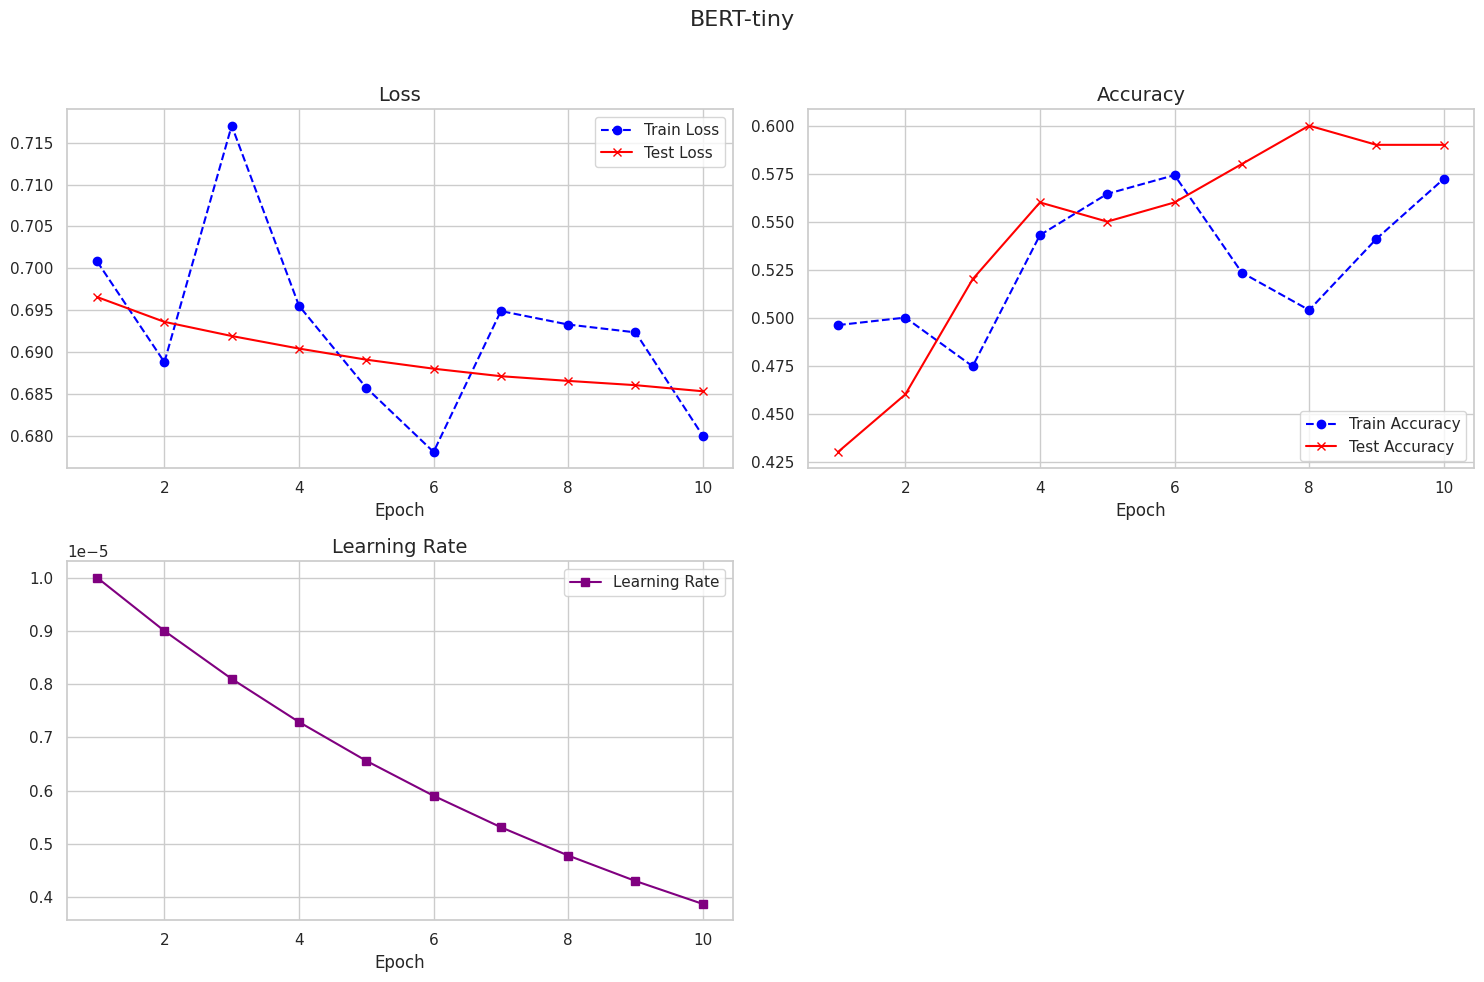
\includegraphics[width=\linewidth]{"C:/Users/alepa/Desktop/Plots/bertiny.png"}
	\caption{Performance of BERT-tiny}
	\label{fig:bert-tiny}
\end{figure}

\subsection{BERT-large}
BERT-large was instead pre-trained on a much more extensive corpora including the entire English Wikipedia and the Brown Corpus, and it amounts to 340 million parameters, which is 85 times more than BERT-tiny. 

We trained BERT-large along 6 epochs since more extensive training resulted in overfitting. The decreasing losses and increasing accuracy trends were less noisy than BERT-tiny and reached a higher accuracy (about 0.71) with less epochs, but still plateaued at an unsatisfactory rate, indicating the need of a architectural change in the model.

\begin{figure}[h]
	\centering
	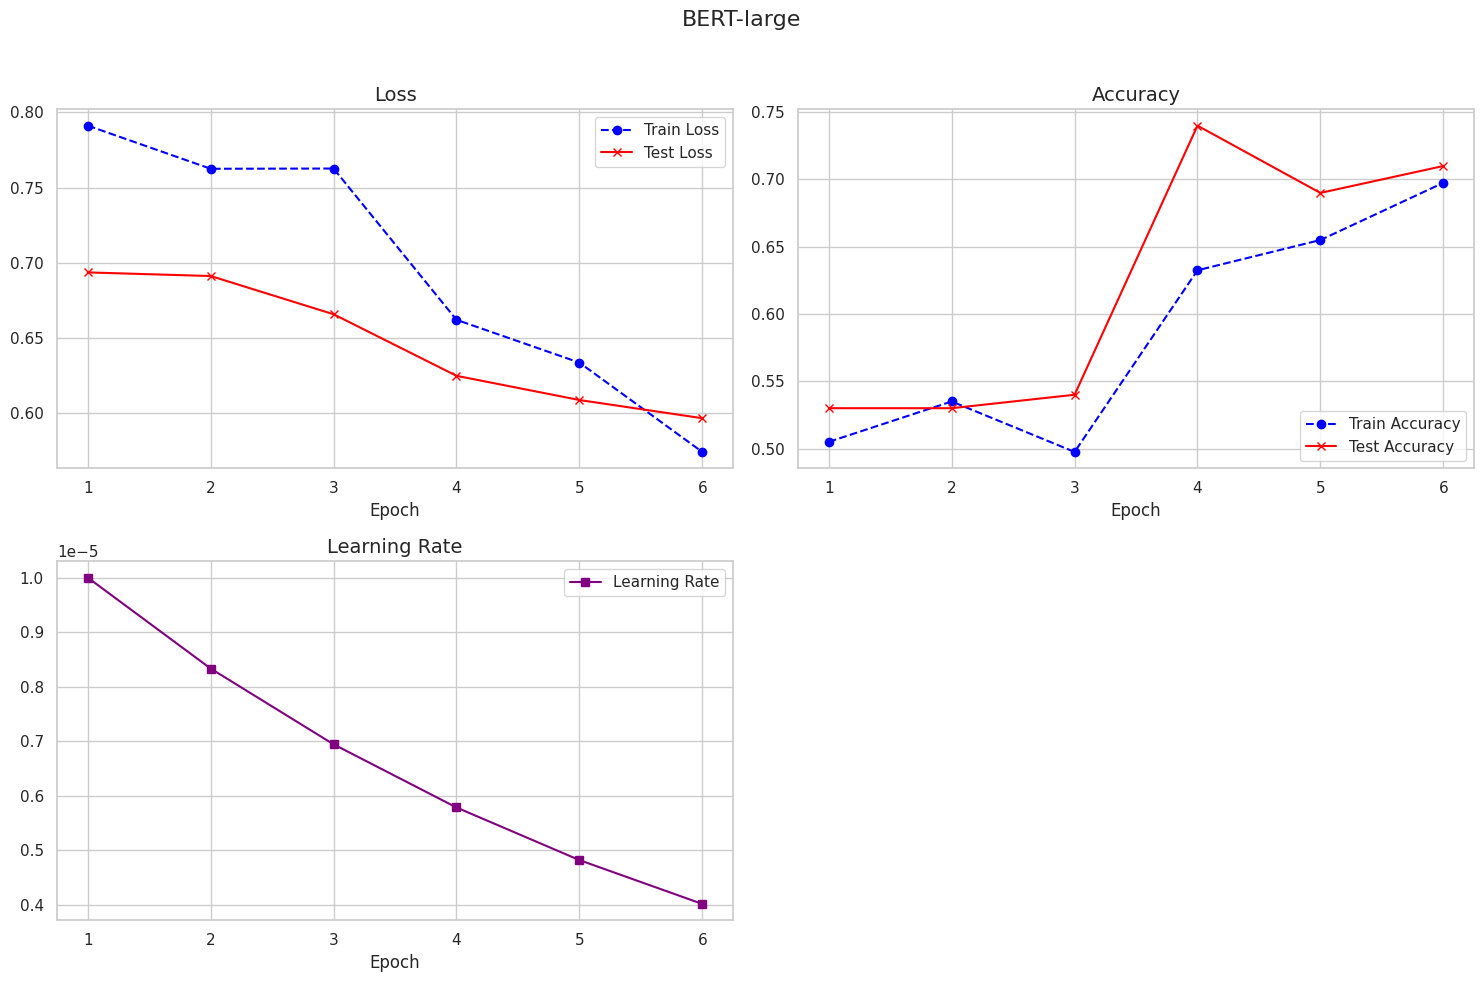
\includegraphics[width=\linewidth]{"C:/Users/alepa/Desktop/Plots/bertlarge.png"}
	\caption{Performance of BERT-large}
	\label{fig:bert-large}
\end{figure}


\subsection{GPT-2}
GPT-2 is instead decoder-only. It is an autoregressive model, meaning it is trained by trying to predict the next word in a sequence without masking, which considers only the leftwards context (preceding words) during prediction \cite{radford2019language}.

We trained GPT-2 for 5 epochs. Trends in loss indicate slight to no improvement, since the test loss only decreased slightly in comparison to the training loss. The accuracy trends also show that the model is not efficacious, since test accuracy is extremely noisy and within low bounds (0.50 to 0.64) and training accuracy increases steadily.

The model’s architecture, designed for text generation, struggles with distinguishing between useful information and noise. This limitation is underscored by the comparison with BERT, which is bidirectional and utilizes the encoder stack, where GPT-2's 'decoder-only' design, lacking the full contextual comprehension of an 'encoder-only' model, proves less effective for this specific task. Hence, we find unwise to adapt GPT-2 for tasks beyond its primary design, text generation.

\begin{figure}[h]
	\centering
	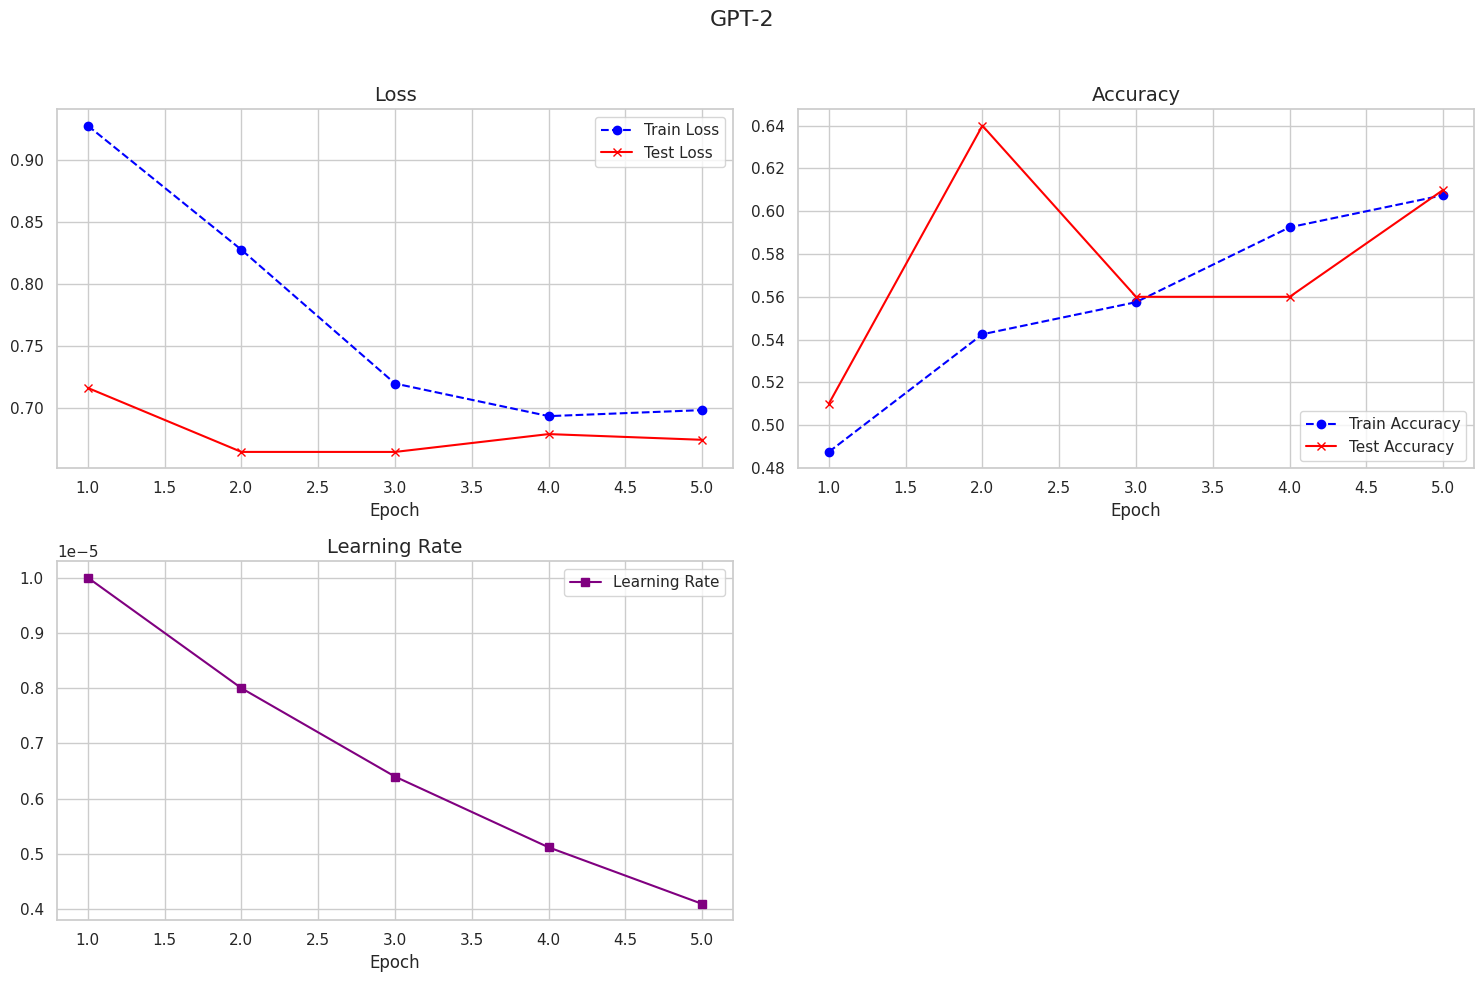
\includegraphics[width=\linewidth]{"C:/Users/alepa/Desktop/Plots/gpt2.png"}
	\caption{Performance of GPT-2}
	\label{fig:gpt-2}
\end{figure}


\subsection{RoBERTa-large}
RoBERTa (Robustly optimized BERT approach) enhances BERT by optimizing the training process, expanding the dataset, and making key improvements such as increasing batch sizes, using dynamic masking, and eliminating the next sentence prediction task \cite{brown2020language}.
We trained RoBERTa for 8 epochs. The model outperformed all the previous ones and reached high accuracy (about 0.88), making it the best and the only model of choice for the task.

\begin{figure}[h]
	\centering
	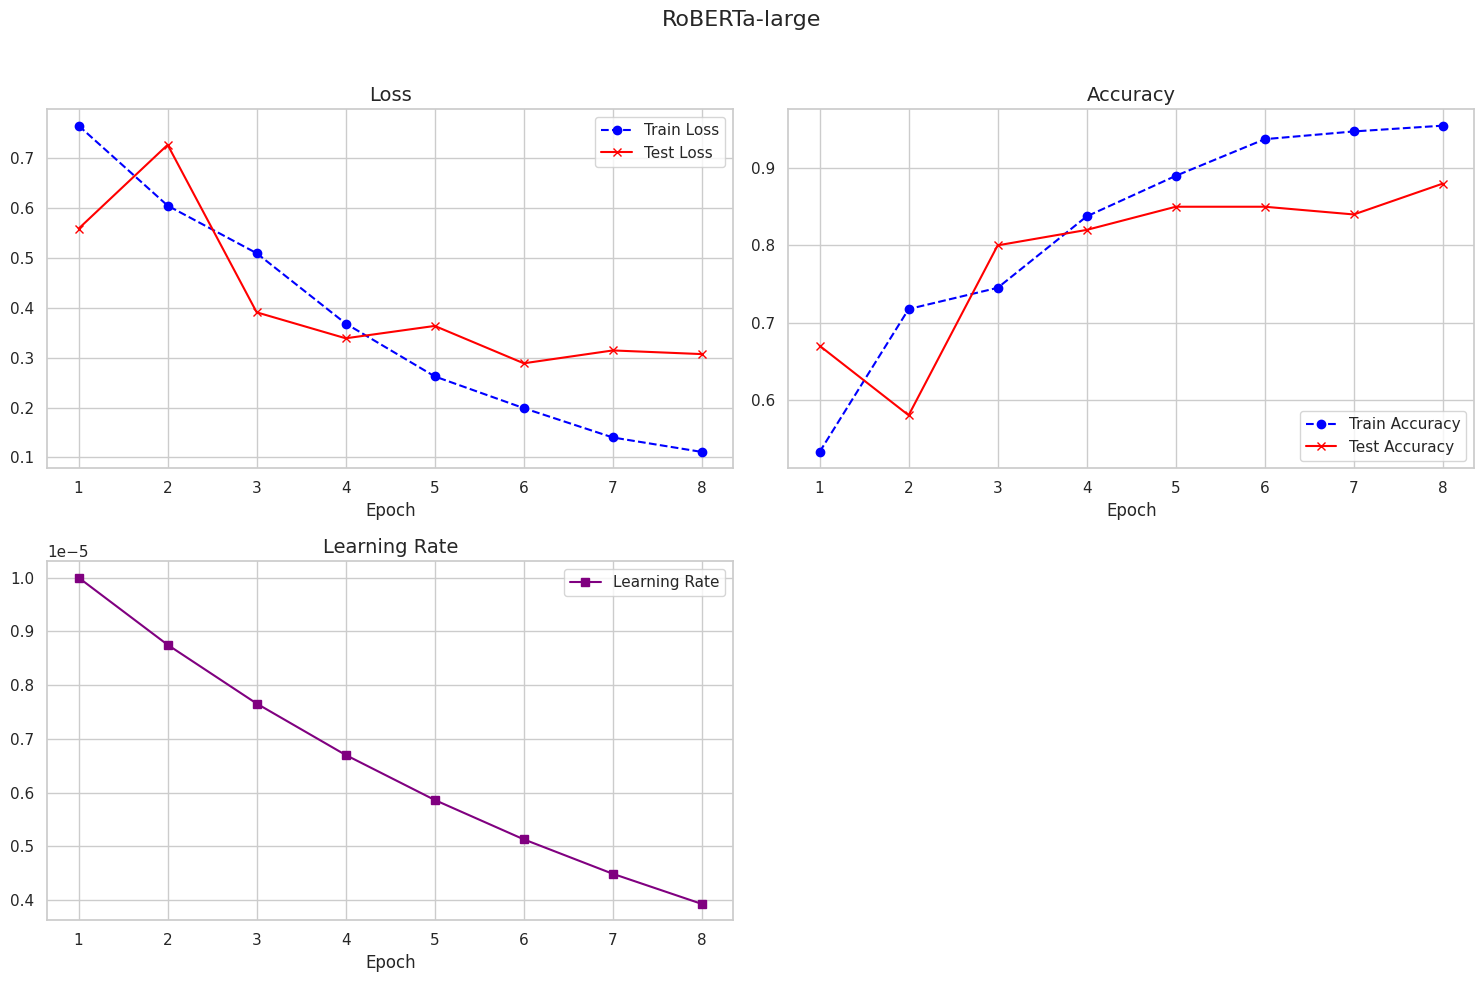
\includegraphics[width=\linewidth]{"C:/Users/alepa/Desktop/Plots/robertalarge.png"}
	\caption{Performance of RoBERTa-large}
	\label{fig:roberta-large}
\end{figure}


\subsection{Summary of the Data}

RoBERTa-large achieved the highest accuracy - 0.88 - and the lowest loss - 0.2 - but had the longest training time (253.2 seconds). BERT-large followed with an accuracy of 0.71, a loss of 0.57, and a training time of 182.5 seconds. GPT-2 and BERT-tiny had lower accuracies (0.61 and 0.59, respectively) and similar losses (0.67 and 0.68, respectively), with GPT-2 training slightly slower - 65.0 seconds - than BERT-tiny (47.8 seconds).

\begin{table}[H]
\begin{center}
\begin{tabular}{|l|c|c|c|c|}
\hline
Model & Accuracy & Loss & Training Time\\
\hline\hline
BERT-tiny & 0.59 & 0.68 & 47.8 s\\
BERT-large & 0.71 & 0.57 & 182.5 s\\
GPT-2 & 0.61 & 0.67 & 65.0 s\\
RoBERTa-large & 0.88 & 0.2 & 253.2 s\\
\hline
\end{tabular}
\end{center}
\caption{Performance of different models on the classification task.}
\label{Table_2}
\end{table}

As mentioned in the Inductive Bias section, any model's accuracy suffers inherently from its structure, the varying degrees of semantic populism in the positively labelled speeches. Hence a best accuracy of around 90\% is about the highest tier achievable given the small dataset, batch size and computing power.

\section{Conclusion}

In this project, we fine-tuned four pre-trained language models to classify speeches as populist or non-populist. Our experiments demonstrated that RoBERTa-large achieved the highest accuracy (88\%), establishing it as the most effective model for this task. This finding suggests that large, encoder-only pre-trained models, particularly those optimized for robust performance like RoBERTa, are highly suitable for binary classification tasks involving nuanced textual analysis, outperforming generative models in this context. Future work should focus on expanding the dataset size to enhance the generalizability of the predictive model. With a larger dataset, it would be possible to explore alternative model structures and objectives, such as training the model to assign multiple labels that represent varying levels of populism, rather than a simple binary classification.

\break

%%%%%%%%% REFERENCES
{\small
\bibliographystyle{unsrt}
\bibliography{egbib}
}

\end{document}
